\chapter{Introduction}

\section{Langevin Equations}

\subsection{The Langevin Equation} \label{sec:langevin_equation}

The Langevin equation provides a mechanism for studying certain complex many-body systems by focusing in on a single particle and treating the effect of other particles as stochastic. Following the derivations of Kubo \cite{Kubo}, this approach leads to the Langevin equation, a stochastic differential equation of the form 
\\
$$
m\ddot{\vec{r}}(t) + m \eta \dot{\vec{r}}(t) = \vec{f}(t)
$$
\\
where $\vec{r}(t)$ is the trajectory of a particle of mass $m$, $\eta$ is a friction constant in units of inverse time and $\vec{f}(t)$ is a stochastic force. It is often assumed that $\vec{f}(t)$ is isotropic, as well as uncorrelated for different times and directions. This is summarized through the relation 
\begin{equation}
\left<f_i(t)f_j(t')\right>=\sigma^2\delta(t-t')\delta_{ij} \label{eq:tdomain_corr}.
\end{equation}
The standard deviation $\sigma$ is given by the fluctuation dissipation theorem \cite{Kubo}, $\sigma^2=2k_BTm\eta$ where $k_B$ is the Boltzmann constant and $T$ is the temperature of the system. The friction term $m \eta \dot{\vec{r}}(t)$ counteracts the energy gain from the stochastic force to ensure the equipartition theorem holds. 

\subsection{The Generalized Langevin Equation}

Some of the assumptions made in the formulation of the Langevin equation do not hold for most real systems. The Fourier transform of \ref{eq:tdomain_corr} results in the expression
\begin{equation}
\left<\tilde{f}_i(\omega)\tilde{f}_j(\omega')\right>=2\pi\sigma^2\delta(\omega+\omega')\delta_{ij}. \label{eq:wdomain_corr}
\end{equation}
This equation tells shows that the power spectrum of the noise force is constant and does not fall off as $\omega \rightarrow \infty$. While this may be a reasonable approximation for many systems, all real system are band limited and therefore exhibit `colored' noise. One may introduce colored noise into the Langevin equation while maintaining the relations \ref{eq:tdomain_corr} and \ref{eq:wdomain_corr} by convolving $\vec{f}(t)$ with a memory kernel $K(t)$. The second fluctuation dissipation theorem \cite{Kubo}, requires a corresponding modification to the friction term which gives us the generalized Langevin equation (GLE)
\begin{equation}
m\ddot{\vec{r}} + m \eta \int dt' K\left(t-t'\right) \dot{\vec{r}}(t') = \int dt' K\left(t-t'\right) \vec{f}(t').
\end{equation}

\subsection{Including Background Potentials} \label{sec:gle_with_background}

If one views the GLE as simple stochastic generalization of Newton's second law, it is simple to add a term to the GLE to include the effect of a position dependent background potential $V(\vec{r})$,
\begin{equation}
m\ddot{\vec{r}} + m \eta \int dt' K\left(t-t'\right) \dot{\vec{r}}(t') + \nabla V\left(\vec{r}\right)= \int dt' K\left(t-t'\right) \vec{f}(t').
\end{equation}
\\
While this approach is very straight forward, it is not immediately obvious that the relation $\sigma^2 = 2k_BTm\eta$ guarantees thermalization in the presence of an arbitrary background potential. The various derivation of the GLE \cite{Kubo, Pathria, Tong} focus exclusively on the case of $V(x)=0$. Nevertheless, Langevin equations are frequently used in contexts where background potentials are necessary and justification for their use is either omitted or provided retroactively through comparison of results with independent sources \cite{Ward, Townsend, AVIDOR2019145}.  

\section{Surface Dynamics and Helium Spin-Echo Microscopy}

The field of surface dynamics aims to measure and model the motion of particles (referred to as `adatoms') adsorbed on the surface of various solid crystalline materials so as to better understand processes such as catalysis or the production of nanomaterials \cite{B810769F}. The field has adopted simulations of the GLE as a computationally efficient tool for studying its dynamical processes \cite{Ward, Townsend, AVIDOR2019145}. The rich experimental data available in the literature provides a setting in which the GLE can be applied to the same system across a wide range of length and time scales \cite{JARDINE2009323, HSEM}.

\subsection{The Cambridge Helium Spin-Echo Spectrometer}

\begin{figure}
	\centering
	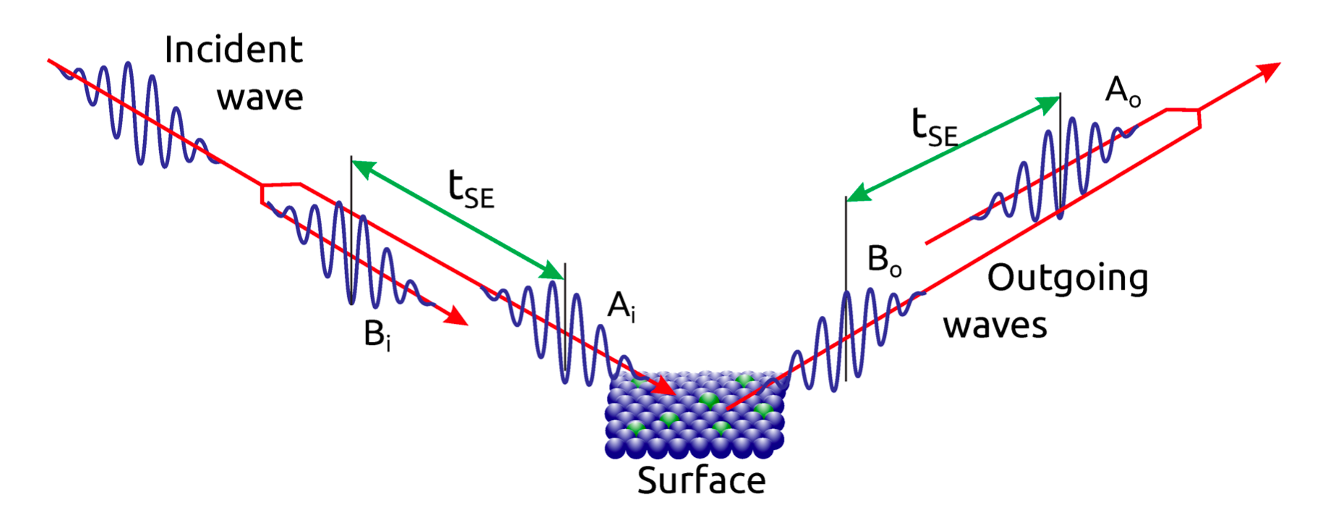
\includegraphics[width=0.8\textwidth]{hsem_schematic}
	\caption{Schematic of the helium spin-echo technique sourced from \cite{B810769F}. An incident spin-polarized helium wave packet is split into two components which strike the surface at distinct times separated by $t_{SE}$. Motion of the adatoms on the surface which occurs in this time affect the polarization of the scattered helium which may be used to construct the ISF of the motion.}
	\label{fig:hsem}
\end{figure}

The Cambridge helium spin-echo spectrometer probes the dynamics of adsorbates on the surface of a substrate using a beam of He-3 atoms scattered off the substrate surface. The spectrometer provides a measurement of the so called intermediate scattering function (discussed further in Section \ref{sec:isf_intro}) of an adsorbate's motion. The core principles of helium spin-echo microscopy (HSEM) are summarized in Figure \ref{fig:hsem} and its implementation is explored in further detail in \cite{Ward, HSEM, JARDINE2009323}.

\subsection{The Intermediate Scattering Function} \label{sec:isf_intro}

A quantity of interest in many surface scattering experiments is the so called intermediate scattering function (ISF) \cite{HSEM, JARDINE2009323, Ward}. The ISF is defined in terms of the Van Hove pair correlation function. For a single adatom, the van Hove pair correlation function coincides with the probability, $P(\vec{r}, t)$, of finding the particle at the position $\vec{r}$ at time $t$ given that the particle was present at the origin at $t=0$ \cite{vanhove} \footnote{This definition strictly speaking only applies when a single adatom is present on the surface. For more details see \cite{vanhove}.}. The ISF is then defined as the spatial Fourier transform of $P\left(\vec{r}, t\right)$,
\begin{equation}
	ISF\left(\Delta{\vec{K}}, t\right) = \int d\vec{r} e^{-i\Delta{\vec{K}}\cdot\vec{r}} P\left(\vec{r}, t\right).
\end{equation}
Within the context of a surface scattering experiment, the argument $\Delta{\vec{K}}$ is often referred to as `the momentum transfer' as this quantity corresponds to the momentum transferred to the surface in the process of scattering. The Cambridge HSEM device is largely insensitive to momentum transfer perpendicular to the surface as motion on the surface in this direction occurs at frequencies which exceed its working range \cite{HSEM}. The ISF is therefore often only quoted in terms of the 2D parallel component of the momentum transfer. 

\subsection{Adsorbate Motion}

Although effectively confined to motion on a 2D plane, adatoms may exhibit various sophisticated forms of motion. Typical motion observed in real systems include 2D diffusion, ballistic motion across the surface and hopping between regularly spaced absorption sites \cite{Ward, Townsend}. The type of dynamics an adsorbate exhibits is influenced by factors such as the details of the adsorbate-substrate interaction, the crystalline structure of atoms in the substrate, the temperature of the system as well as the density of the adatoms on the surface \cite{Ward, Townsend}. 

The motion of an adsorbate may vary over different timescales. Consider an adatom which spends most of its time oscillating about its local equilibrium in an absorption site but every so often obtains the energy to jump over to a neighboring absorption site. On short timescales (less than its typical oscillation period), the motion appears Brownian as the adatom randomly moves about the local patch of its potential well. At somewhat larger timescales, the particle will appear to oscillate about its potential well at some frequency approximately given by the curvature of the local equilibrium. On the longest time scales the particle appears to hop between well defined absorption sites. The signature of the motion on the different timescales is imprinted on the ISF and may be extracted with suitable analysis \cite{Ward}.

\pagebreak

\section{Lithium on Copper 111}

\begin{figure}
	\centering
	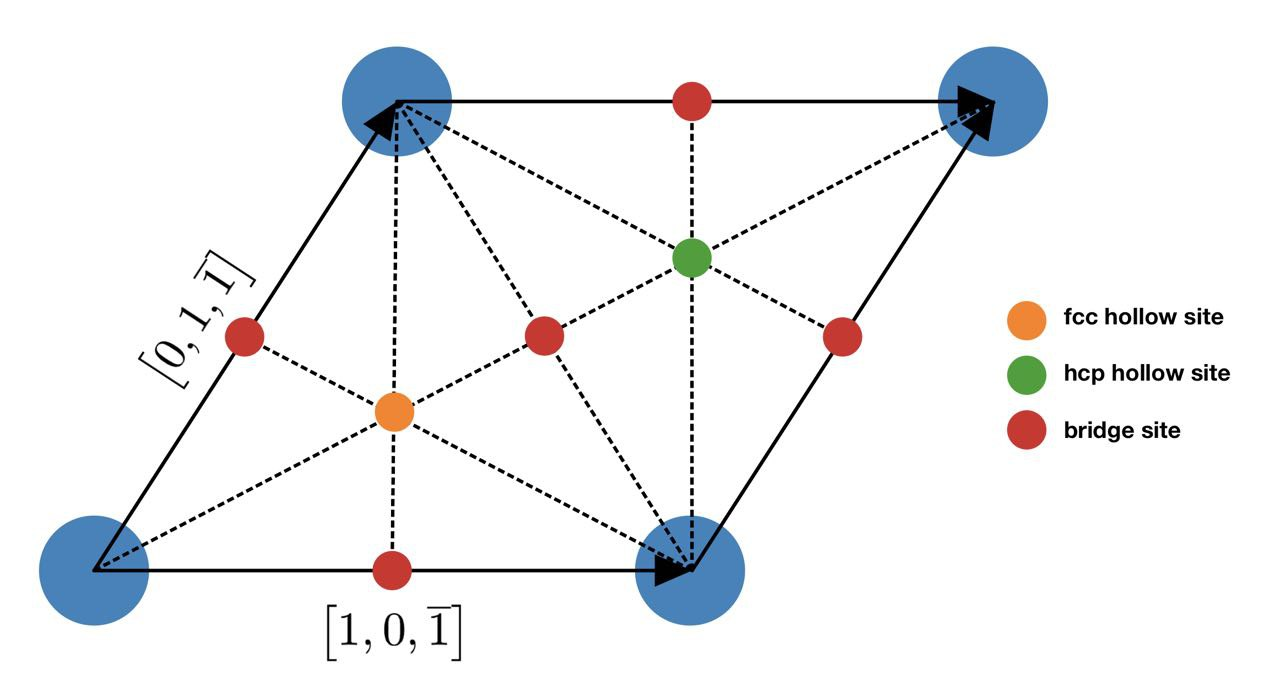
\includegraphics[width=0.8\textwidth]{primitive_cell}
	\caption{The unit cell which tiles a copper(111) surface. Lithium adsorbed on the surface is observed to sit within the two types of hollow sites and hop between sites with an activation energy of approximately $8\mev$ \cite{Ward}.}
	\label{fig:fcc_111_unit_cell}
\end{figure}

Previous work has used the GLE to explain the dynamic processes of Lithium adsorbed on copper(111) \cite{Ward}. Copper crystals have a face centered cubic (fcc) crystal structure and the 111 surface is tiled by the unit cell shown in Figure \ref{fig:fcc_111_unit_cell}. The experimental HSEM ISFs for lithium on copper(111) shows signs of activated diffusion at $\SI{140}{\kelvin}$ and previous work has concluded that the ISFs can be entirely reproduced through a GLE simulation with a band limited noise spectrum \cite{Ward}. The 3D molecular dynamics simulation presented in this report is modeled on this system to investigate the origin of this band limited noise spectrum. 
